\documentclass[10pt,twocolumn]{IEEEtran}

\usepackage[linesnumbered,lined,boxed,commentsnumbered, noend, noline]{algorithm2e}
\usepackage{graphicx}
\usepackage{xcolor}
\usepackage{soul}
\usepackage{supertabular}
\usepackage{tabularx}

\newcommand{\hlc}[2][yellow]{{%
    \colorlet{foo}{#1}%
    \sethlcolor{foo}\hl{#2}}%
}

\title{Analyzing Algorithmic Patterns Based on Real Coding Interview Questions}
\author{\IEEEauthorblockN{Ian Dempsey,\\
Computer Science Department,\\
Maynooth University,\\
Email: ian.dempsey.2013@mumail.ie}
}
%\hlc[cyan!50]{_____} -> put in the stuff to be highlighted inside the {}
%cite{___} ->put in the bibtex key for the specific source.
%\label{sec: | fig: | } -> use to give something a specific label. This allows it to be referenced later
%\ref{___} -> to refernce a previously labeled area
\begin{document}

\maketitle
\pagenumbering{gobble}
\newpage
\pagenumbering{arabic}
\section{Abstract}
This is my abstract. It is empty for now. Fill in later
\section{Introduction}
\label{sec:intro}
\par
Nowadays interviews for jobs in the I.T industry are becoming more complex and demanding on the applicant. As this section of the working industry is usually quite technical, it is quite common for the applicants to have to perform some form of technical test. These tests normally involve a question or two that are based on a wide variety of topics in programming. These questions in particular are used to test potential employees on whether they have strong analytical and critical assessment skills. The technical tests also allow the employer to see how many standard algorithms the candidate knows, and is able to use. However, it is difficult to master all of the different types of algorithms and their intricacies. 
\par The purpose of this paper is to study the relationship between the classical and well known algorithms, and the interview questions which are commonly asked.  This paper aims to give guidance to people who want to study the interview questions, but also learn a core set of common ideas which will help them solve multiple problems. This would therefore allow them to save time as they prepare for the interview.
\par This paper presents a comprehensive report summarising the similarities between interview questions and standard algorithms taught in any programming course. This distinguishes our work from interview preparation books which focus on the problem solving skills, simply showing the reader a solution to a single problem, and not reinforcing material they would already be familiar with. This paper's goal is to show people that understanding the fundamentals of several common algorithms will allow them to be able to solve a wide array of problems. It is also the purpose of this paper that a beginner of programming or a fresh graduate can use this paper as guidance to show them how much time is needed for preparatory work before they have the interview.  
  %The questions themselves have a wide range of difficulty, from easier ones which focus on in basics of programming- e.g., array indexing, sorting algorithms, up to harder questions which really push candidates- e.g., dynamic programming, graphs. This area of interviewing is known as \textit{whiteboarding}, and has become quite common, it has led to some books being published which compile together numerous questions which are popular for interviewers to ask\cite{mcdowell2015cracking}.The focus in this paper is not the ability to solve as many quetions as possible to give to the applicants to study, but to try and discover patterns in problems which are similar, and then classify these patterns based off of pre-established patterns that candidates would be used to. This classification will then be able to help applicants and fellow programmers to learn how to see the patterns in problems quicker and be able to apply them to multiple problems, where they need only alter specific areas of code to solve the target problem. %
\section{Technical Background}
\par Nowadays, in general, there are a lot of online repositories for interview questions and interview related material. Websites such as hackerrank.com, glassdoor.ie, geeksforgeeks.org, and leetcode.com all offer information on what questions are common during interviews for different companies. They also offer ways to test potential solutions to some of the given questions. 
\par For this paper we chose to use leetcode.com\cite{leet1}, as this website comes with a huge amount of online material that is generally taken from previously asked interview questions. Companies also use sites similar to leetcode when they are building up a bank of questions to pose to candidates. This was important in our decision for the repository, as it meant we were using a platform which was regularly updated. LeetCode itself also has some built-in features which greatly appealed to us. The website has an online discussion forum for each question, allowing the community to discuss solutions, issues, and the questions themselves. LeetCode also host their own weekly coding competitions which allow users to gain more experience and confidence in coding problems. One of the unique main features this online judge website has in comparison to others is a section for a user to perform a mock interview. This mock interview is under the time constraint of a normal real world interview, this was a pre-eminent for us in choosing our online judge. The online editor that is used by leetcode also allows a user to select from a multitude of programming languages, as shown in figure \ref{fig:langUI} below. For the purpose of this paper the language that was chosen was java. The reason for this is because it is a language most people learn first. However, any choice of programming language would be just as acceptable, as we present pseudocode throughout the paper which can be used by any major programming language.  
\par The user interface of LeetCode is very simple and accessible to use. The main page which lists all of the problems, offers its users the option to filter questions by difficulty, which company has asked it before, what area the questions focuses on and much more. As seen in figure \ref{fig:homepage}, we have chosen to focus on questions which are tagged as being related to trees. 
\begin{figure}[h]
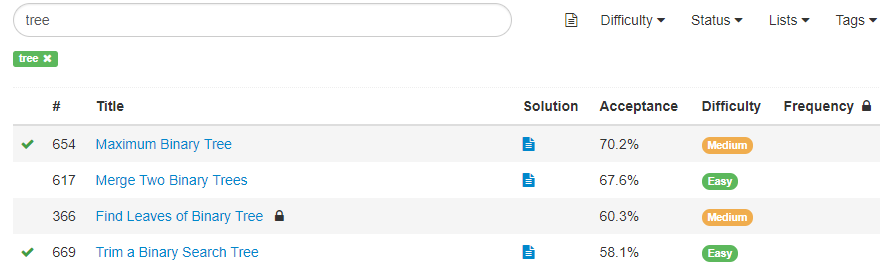
\includegraphics[width=0.5\textwidth]{homepageUI.png}
\caption{Homepage}
\label{fig:homepage}
\end{figure}

A user simply chooses the question which they wish to attempt, and is promptly brought to the problem's specific screen, as seen in figure \ref{fig:problemPage}. On this screen there is a general description of the problem and a few examples for more clarification. This page also contains the online editor that the user will operate to attempt the problem. The online editor is intuitive to understand, and as stated has a variety of options for the user to choose from. 
\begin{figure}[h]
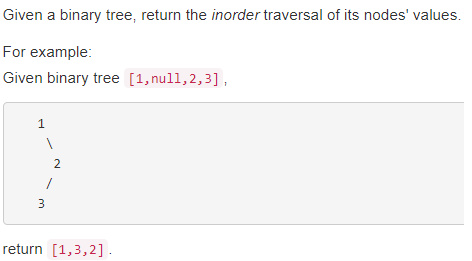
\includegraphics[width=0.5\textwidth]{problemPage.png}
\caption{Problem Specific Page}
\label{fig:problemPage}
\end{figure}

\begin{figure}[h]
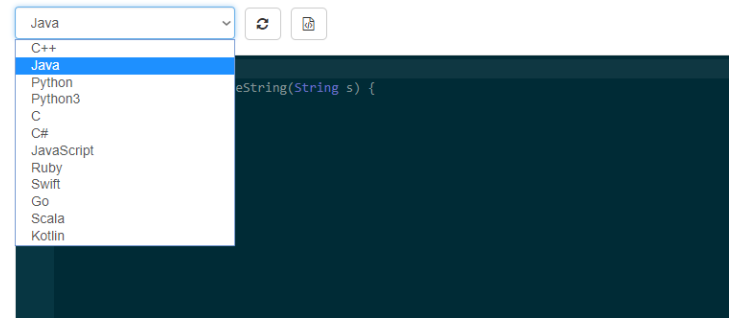
\includegraphics[width=0.5\textwidth]{languageUI.png}
\caption{Online editor with options displayed}
\label{fig:langUI}
\end{figure}   
The user will attempt to solve the problem they have selected, and they will then want to submit their answer and see if it was correct. They perform this by clicking the submit solution button underneath the editor. Leetcode allows a user to sumbit their code and be informed almost instantly if they are correct or not. There are two possible outcomes once the user clicks the submit button. Either it is accepted and leetcode returns an accepted result with suggestions for the next question a user could attempt, shown in figure \ref{fig:accepted}, or their answer failed a certain testcase or even their code failed to compile and run, shown in figure \ref{fig:fail}. In the case of failure, leetcode will report where an error is in the code by referencing the line.  
\begin{figure}[h]
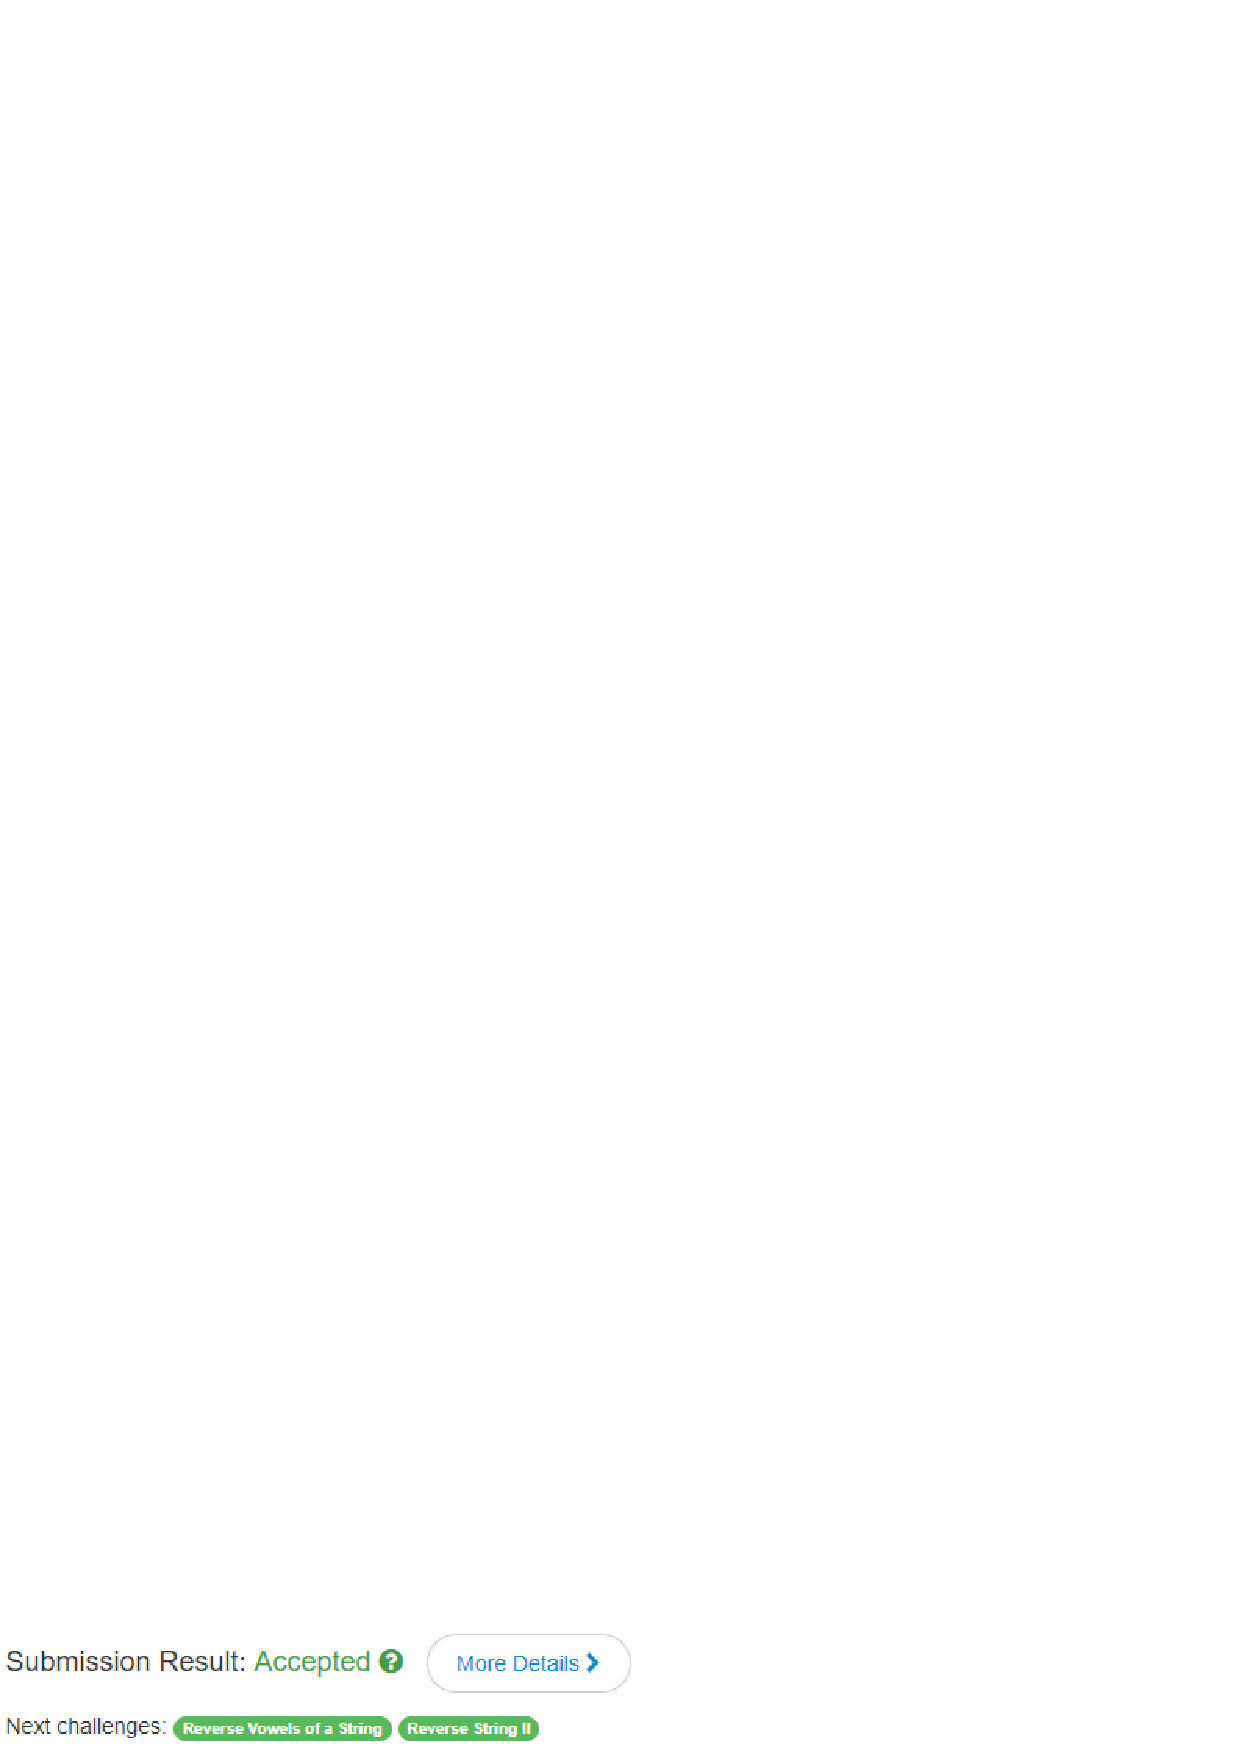
\includegraphics[width=0.5\textwidth]{accepted.png}
\caption{User solution passes all testcases}
\label{fig:accepted}
\end{figure}  
\begin{figure}[h]
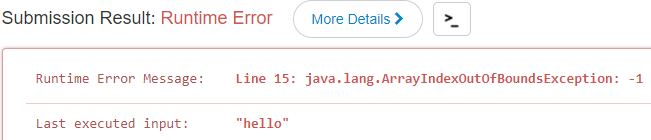
\includegraphics[width=0.5\textwidth]{failure.png}
\caption{User solution failing submission}
\label{fig:fail}
\end{figure}    

\section{Problem Statement}
In order to fulfill the goal of this paper, we will answer the following research questions:
\begin{enumerate}
\item What algorithms to choose, and what categories are these algorithms associated with. 
\item How do these algorithms relate to the classic algorithms and how similar are they.
\item How easy is it for a person to indentify the pattern of the algorithm.
\end{enumerate}
\section{The Solution}
To answer question one above, we had to perform some information gathering. Many companies choose similarly styled questions for their technical tests, so we gathered information from forums, such as glassdoor.ie \cite{glassdoor}, and websites which discussed experiences people had at interviews. We also read through the main categories listed in books which prepare people for interviews, such as Cracking the Coding Interview \cite{mcdowell2015cracking} These discussions listed the questions they were asked, and by what companies. The website geeksforgeeks.org has a list of the top interview questions that a user should study prior to an interview \cite{geeksalgos}. Therefore this paper focuses on the following areas:
\begin{itemize}
\item Sorting Algorithms
\item Searching Algorithms
\item Graphs
\item Trees
\item Dynamic Programming
\end{itemize}
In each of these areas we categorised them into some key patterns. These are patterns or types of the above listed algorithms which commonly appeared. These include, but are not limited to:
\begin{itemize}
\item Palindrome
\item Merge Sort
\item Binary Search
\item Tree Traversal
\item Breadth-First Search
\item Depth-First Search
\label{itm:patterns}
\end{itemize} 
par Leetcode has over six hundred questions, which is impossible for us to answer in such a short period of time. So we chose a representative amount of this total. We selected them based on reputation, if they were asked in interviews, and the solve rate of the question. Relating back to figure \ref{fig:homepage}, it can be seen that we are able to filter out the questions we chose.
\par With regards to question two above, in order to find the most similar algorithm, we first compared the ideas of the classical algorithm and the solution to the question we were solving. It is possible to have multiple algorithms apply to a problem. We implemented the easiest solution which is the first which came to our minds. This is because one normally has limited time in an interview, and this means that a person would build on an idea they initially discover after they understand the question being asked. The candidate would not have enough time to explore multiple solutions to a problem under the interview conditions. We also compared a control flow graph of our solution, in comparison to the standard algorithm. We have listed the aformentioned patterns in the following section, along with sample questions which are similar to the classical algorithms. We picked only a few to represent all of the questions due to the page limit. Please see table \ref{tab:tabSols} for more detail.  	 
\subsection{Palindrome}
Palindromes are extremely useful for searching algorithms, as Palindromes are meant to be the same in both directions, one can easily discover if the input is an actual palindrome. This is helpful for searching because one can search and find the odd character out, or the unique piece of data in some text. This style of algorithm is also space efficient, they normally have a space analysis of O(n/2) as the algorithm works over two elements of the input at a time. The basic approach of a Palindrome algorithm is to work inwards with both pointers starting at either end of the input and constantly moving towards one another and comparing if the elements are the same.\\  
The following description is a general algorithm for solving the palindrome problem which is a common problem in Java and other languages. This approach can be used to solve numerous other problems by altering the inside of the loop.
Pseudocode:
\IncMargin{1em}
\begin{algorithm}
	\SetAlgoLined
	\SetKwInOut{Input}{Input}
	\SetKwInOut{Output}{Output}
	\Input{Given input of characters, S}
	\Output{Boolean}
	$leftIndex  \longleftarrow $S[0]\;
	$rightIndex \longleftarrow $S.length-1\;
	\While{leftIndex $<$ rightIndex}{
	
	compare leftIndex with rightIndex\;
	\If{leftIndex !=rightIndex}{
		return false\;
	}
	 leftIndex++\;
	rightIndex++\;
}
return true\;
\caption{The Palindrome Algorithm}
\end{algorithm}\DecMargin{1em}

Whilst studying and working on this project, we have answered a number of questions from Leetcode.com which we where able to solve using an altered version of the above Palindrome pattern. \textbf{ID 1} TwoSum is one example. This question is described as: \textit{Given an array of integers, return indices of the two numbers such that they add up to a specific target. You may assume that each input would have exactly one solution, and you may not use the same element twice.} The following pseudocode is our answer to this question. In it we have taken the basic idea of the Palindrome algorithm of having two pointers used for looking through the input data, but we have altered the way these two pointers behave.In this pseudocode we have highlighted any differences in blue.
\IncMargin{1em}
\begin{algorithm}
	\SetAlgoLined
	\SetKwInOut{Input}{Input}
	\SetKwInOut{Output}{Output}
	\Input{Array of integers nums, target S}
	\Output{Indices i,j}
	$leftIndex  \longleftarrow $S[0]\;
	$rightIndex \longleftarrow $S.length-1\;
	\While{leftIndex $<$ rightIndex}{
	\hlc[cyan!50]{Sort the input array nums\;}\\
	\uIf{\hlc[cyan!50]{nums[leftIndex]+nums[rightIndex] $>$ S}}{
		\hlc[cyan!50]{rightIndex$--$\;}
	}\uElseIf{\hlc[cyan!50]{nums[leftIndex]+nums[rightIndex]$<$S}}{
		\hlc[cyan!50]{leftIndex++\;}
	}\Else{
		\hlc[cyan!50]{return leftIndex, rightIndex\;}
	}
     }return 0\;
\caption{LeetCode Q1 TwoSum}
\end{algorithm}\DecMargin{1em}\\
As can be seen from the above answer, the main differences are the conditionals inside the while loop. Instead of the normal approach of a Palindrome where one checks if the two elements are equal, and if so moves the two pointers are moved at the same time towards eachother, we have changed the conditionals such that instead of moving both of these pointers together at the same time, we only ever move one pointer at a time. Depending on the result of adding the two current elements at each pointer together. If the total from adding the two integers together was greater than the target sum, then we knew that we had to move the right-pointer left once, as this would allow us to have a smaller sum and potentially the correct sum. If on the other hand the sum was smaller than the total, we would only move the left-pointer right once and add the two elements and get a new result. This process was repeated until the target sum was found, or until the two pointers crossed which meant the target was not found.
\subsection{Merge Sort}
Merge Sort is a very powerful algorithm. It is more efficient than most styles of insertion, with a time analysis of $O(n * log_{n})$, whereas insertion is $O(n^2)$. The idea of merge sort is to divide an array or some input in half and then sort each half before joining it back together. They do not have to be the same size which is useful.  \\
Merge Sort uses the idea of divide and conquer, this means the list to be sorted should be divided up into equal parts first, then these new smaller parts should be sorted individually first before recreating the full list.
Pseudocode:
\IncMargin{1em}
\begin{algorithm}
	\SetAlgoLined
	\SetKwInOut{Input}{Input}
	\SetKwInOut{Output}{Output}
	\Input{List of unsorted data}
	\Output{Sorted List}
 	\eIf{ length of A is 1}{ return 1}
  	{Split A into two halves , L and R. Repeat until size of part =1\\
  	Sort each part individually \\
  	Merge with another subdivided section into B, the sorted list\\ 
  	Return B, the sorted structure}
\caption{The Merge Sort Algorithm through Recursion}
\end{algorithm}\DecMargin{1em}

	\subsection{Graphs}
	Graphs are common in our lives. News media use them to help us visualize certain statistics. Though these are not the graphs that are studied by Computer Scientists. Graphs studied by Computer Scientists are usually based on the tree structure, and the relationships 	among data elements. A tree is just one of the special types of graphs that can be studied, where the parent-child relationship is used to organise data. In this section I have focused on the Tree Abstract Data Type, Breadth-First Traversal, Depth-First Traversal and Graphs in general. \\
	\subsubsection{Trees}
	Trees are one of the most powerful styles of data structures for processing data, this is because they allow rapid searching and fast insetion/deletion of a node. Trees are made up of nodes, these are Objects which hold some data and have a key. This key allows one to determine where this node should be in the tree. The important distinction here with these nodes in comparison to other nodes used in various data structures, is that these nodes contain references to children instead of just the next Link. Each node has exactly one parent, but can have many children.A Binary Tree is a special type of tree, this is a tree which has between 0 and 2 children. The first node in a tree is the Root, and it is possible to traverse to any node in the tree from this node.
	With trees the main function is traversal. There are three basic styles of traversal: inorder, preorder and postorder. Inorder visits every Node in ascending order based on their key values. Preorder is where the root is visited first, followed by it's left subtree and then it's right subtree. Finally, postorder is where the left subtree is followed by the right subtree and then the root. \\
The following is an example of how one might search for a particular Node in a Tree.\\
Pseudocode:
\IncMargin{1em}
\begin{algorithm}
	\SetAlgoLined
	\SetKwInOut{Input}{Input}
	\SetKwInOut{Output}{Output}
	\Input{Given a key to search for}
	\Output{The desired Node, or null}
	$Node current \longleftarrow$root\;
	\While{current.data is not key}{
		\If{current is null}{return null\;}
		\eIf{current.data $>$ key}{
			move left on the tree\;
		}{
		move right on the tree\;
		}
	}
return current\;
\caption{Finding a specific Node in a tree based on the key}
\end{algorithm}\DecMargin{1em}
\\
\IncMargin{1em}
\begin{algorithm}
	\SetAlgoLined
	\SetKwFunction{postOrder}{postOrder}
	\Indm\postOrder{$Node localRoot$}
	%\SetKwInOut{Node localRoot}
	%\SetKwInOut{Print out in PostOrder}
	\\
		\If{localRoot $!=$ null}{
		\postOrder(localRoot leftChild)\\
		\postOrder(localRoot rightChild)\\
		Print(localRoot data)\;}	
\caption{Basic Tree Traversal using PostOrder Traversal}
\end{algorithm}\DecMargin{1em}
\\
\textbf{ID 104}, \textit{Maximum Depth of Binary Tree}, is an example of a problem where we used the basic tree traversal styles to solve the question.The problem description is given as: \textit{Given a binary tree, find its maximum depth.The maximum depth is the number of nodes along the longest path from the root node down to the farthest leaf node.} In this algorithm we used postorder traversal. Pseudocode can be found in Algorithm 6 of this paper.\\
\IncMargin{1em}
\begin{algorithm}
	\SetKwFunction{maxDepth}{maxDepth}
	\Indm\maxDepth{$TreeNode  localRoot$}\\
	
	%\SetKwInOut{Node localRoot}
	%\SetKwInOut{Print out in PostOrder}
		\If{\hlc[cyan!50]{localRoot $==$ null}}{\hlc[cyan!50]{ return 0\;}}
		\hlc[cyan!50]{int ldepth $=$}\maxDepth(localRoot leftChild)\;
		\hlc[cyan!50]{int rdepth $=$}\maxDepth(localRoot rightChild)\;
		\If{\hlc[cyan!50]{ldepth $>$ rdepth}}{
		\hlc[cyan!50]{return ldepth+1}
		}\Else{\hlc[cyan!50]{return rdepth+1}}
\caption{Leetcode Q104 Max. Depth of Binary Tree}
\end{algorithm}\DecMargin{1em}
\\
As highlighted above, the key diference is inside the if statement. We changed the conditional itself as it is the base case to stop the recursive execution. We created a variable \textit{ldepth} which is the total depth of the left subtree. This is a recursive call on the leftChild of the current node. Line 4 will execute until it can't go left anymore, if it reaches null it will try to go right once, and then return going left. This is repeated until both calls return null. It will then go back all the way up until we reach the first call to go left, and set this summation of steps to ldepth. It then performs this same process but on the right subtree of the current node(which is the original node given), and set it to the variable \textit{rdepth}. Finally there is a conditional checking if ldepth is greater than rdepth. If so it returns ldepth+1,or it returns rdepth+1. This+1 is required as we need to take into account the root node's level, if we didn't take this into account my answer would always be one less than the actual depth of the tree. The major similarities between the postorder algorithm and this solution is the way we went down the left subtree first, then the right subtree and finally to take the root into account we added one to the height. This particular way of traversing the tree, left-right-root, is exactly how postorder traversal is performed.
\\
\subsubsection{Breadth-First Traversal}
This is a special way to visit the nodes in a tree, the ordering in this traversal pattern is to visit the root node, then move onto the children of the root node, printing each child in turn. It then will repeat this for each child of these nodes.Figure 1 shows the nodes in numerical order of visitation when using Breadth-First Traversal. \\
\begin{figure}[h]
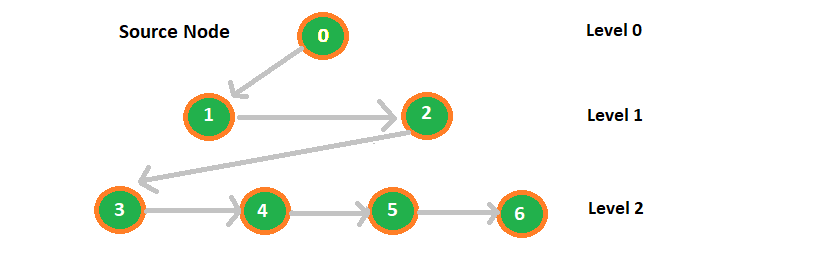
\includegraphics[width=0.6\textwidth]{bfs.png}
\caption{Breadth-First Traversal}
\end{figure}
 \\
\subsubsection{Depth-First Traversal}
This is a second way of visiting nodes in a tree. This pattern involves starting at the root node, then going to the left most child, then repeating this movement until the traversal reaches a leaf node (a node which has no children), then it will move back up one node and try to visit the next child node of this current node. It repeats this until the traversal finds no univisited node. Figure 2 shows the nodes in numerical order of visitation when using Depth-First Traversal. 
\begin{figure}[h]
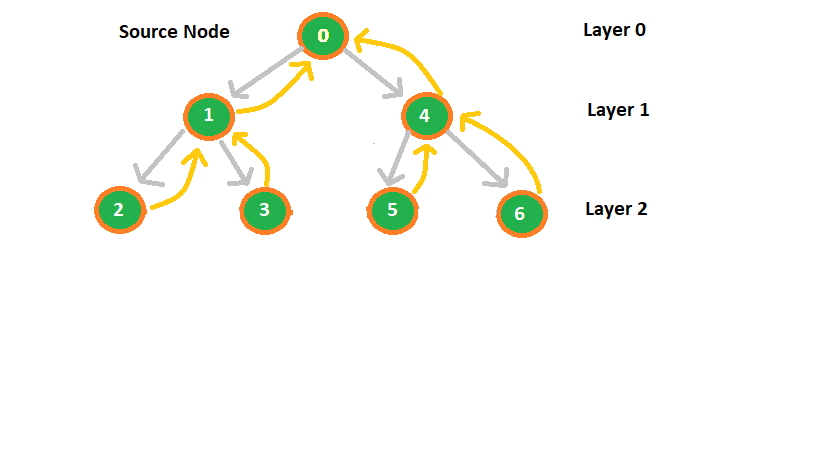
\includegraphics[width=0.6\textwidth]{dfs.png}
\caption{Depth-First Traversal}
\end{figure}

\subsection{Dynamic Programming}
Dynamic Programming is often referred to as `smart recursion'. This is because it takes the idea of recursion and improvess the inefficiencies that come along with it. These inefficiencies mainly being that recursive algorithms are generally space inefficient. Each recursive call adds a new layer to the stack. This is why dynamic programming is such a strong style of programming. It is normally just a matter of taking a recursive algorithm and finding the overlapping subproblems. A user then caches these results for future recursive calls.
This style is known as \textit{Top-Down}. There is a different approach, known as \textit{Bottom-Up}. We will give a quick demonstration of the two by using the classic recursive algorithm to solve Fibonacci numbers.
\IncMargin{1em}
	\begin{algorithm}
		%\Fn(\tcc*[h]{recursive fibonacci}){\FRecurs{Integer n}}{
		\SetKwInOut{Input}{Input}
		\SetKwInOut{Output}{Output}
		
		\Input{Integer n}
		\Output{Fibonacci Numbers}
		\If{n$<$3} {return 1\;}
		return fib(n-2) + fib(n-1)\;
			
	\caption{Fibonacci Numbers through normal recursion}
	\end{algorithm}
\DecMargin{1em}
	
	\subsubsection{Top-Down}
	This method of dynamic programming is known as top-down as we would follow the normal structure of a simple recursion solution, we start from n and compute smaller results as we need them in order to solve the original problem. We then store these results in some 		form of data structure, this is known as memoization. We can then access these results quickly and efficiently in comparison to having to recompute the same values for n over and over again. This leads to us saving space and time when working with recursively styled 		problems. Though it is not the most efficient still. 
	
\IncMargin{1em}
	\begin{algorithm}
		\SetKwInOut{Input}{Input}
		\SetKwInOut{Output}{Output}
		\Input{Integer n}
		\Output{Fibonacci Numbers}
		$computed \leftarrow $HashMap\;
		\If{n$<$3} {return 1\;}
		return fib(n-2) + fib(n-1)\;
		computed put (1,1)\;
		computed put (2,1)\;
		return fib2(n, computed)\;
		\caption{fib; Fibonacci Numbers through Top-Down and Memoization}
	\end{algorithm}\DecMargin{1em}
\IncMargin{1em}
	\begin{algorithm}
		\SetKwInOut{Input}{Input}
		\SetKwInOut{Output}{Output}
		\Input{Integer n, HashMap computed}
		\Output{Fibonacci Number}
		\If{computed containsKey(n)} {return computed get(n)\;}
		computed.put(n-1,fib2(n-1,computed))\;
		computed.put(n-2,fib2(n-2,computed))\;
		$newVal \leftarrow $computed.get(n-1) + computed.get(n-2)\;
		return newVal\;
	\caption{fib2;Fibonacci Numbers through Top-Down and Memoization}	
	\end{algorithm}\DecMargin{1em}	
	
	
	\subsubsection{Bottom-Up}
	The issue with this memoized version is that even when we are saving the results to resue them later, we still have to go all the way down to the base cases with the recursion the first time. This is when we have yet to compute any values, so we have nothing stored.
	Bottom-Up solves this by going in reverse to the normal recursive way. Instead of going down to the base case from the value of n, it works its way up to the value of n.   
\IncMargin{1em}
	\begin{algorithm}
		\SetKwInOut{Input}{Input}
		\SetKwInOut{Output}{Output}
		\Input{Integer n}
		\Output{Fibonacci Numbers}
		\SetKwArray{Kw}{results}
		$results[] \leftarrow $int[n+1]\;
		results[1] = 1\;
		results[2] = 2\;
		\For{$i \leftarrow 3$ \KwTo $n$}{ 
		results[i] = results[i-1]+results[i-2]\;}
		return results[n]\;		
		\caption{fibDP; Fibonacci Numbers through Bottom-Up}
	\end{algorithm}\DecMargin{1em}
\par It must be noted though that Dynamic Programming is one of the toughest sections of programming to learn. This only makes it more challenging for candidates to answer questions in interviews in such a limited window. The reason it is so tough is because a candidate must think of the problem in mutliple ways, and make the decision to tackle it in a certain way. If they choose the wrong option, then they will end up with a very inefficient solution, choose correctly and they will have shown a very strong understanding of this area.
\section{Evaluation}
In the previous section of this paper, we only gave specific examples of the questions that we answered. Here we give a detailed summary of all solved questions in table \ref{tab:tabSols}. All of these were accepted by leetcode's online judging system. 
We also have created a table which details a numeric value for the algorithms previously listed in \ref{itm:patterns}.
\begin{table}[t]
\centering
	\begin{tabular}{| c | c |} \hline
		    &Algorithm \\ \hline
		1 & Palindrome\\ \hline
		2 & Merge Sort\\ \hline
		3 & Binary Search\\ \hline
		4 & Tree Traversal \\ \hline
		5 & Breadth-First Search\\ \hline
		6 & Depth-First Search\\ \hline
		7 & Dynamic Programming\\ \hline
		8 & Not Applicable\\ \hline
	\end{tabular}
	\caption{The classical algorithms}
	\label{tab:classicalAlgos}
\end{table}

\begin{table}[t]
 \begin{tabular}{|c| c| c| c| c| c|} \hline
 Question ID & PassRate & Difficulty & Time(mins) &Evaluation &Algorithm \\
	 \hline
 	1 & 36.0\% & Easy & 9 & Easy & 1\\ 
 	\hline
	 2 & 28.1\% & Medium & 20 &Medium& -- \\
 	\hline
	 20 & 33.7\% & Easy & 12&Easy& 1? \\
 	\hline
 	21 & 39.3\% & Easy & 25&Easy& Graphs(?) \\
 	\hline
 	23 & 27.7\% & Hard & 27&Medium&2 \\
  	\hline
 	35 &39.8\%  & Easy & 10 &Easy&Linear Search\\
  	\hline
 	53 &39.9\%  & Easy & 20 &Medium&Array\\
  	\hline
 	58 & 32.0\% & Easy & 15 &Easy&String/Array\\
  	\hline
 	69 & 28.2\% & Easy & 19 &Easy&3\\
  	\hline
 	70 & 40.5\% & Easy & 18 &Easy&7\\
 	\hline
 	72 & 32.1\% & Hard & 29 &Hard&7\\
  	\hline
 	88 & 32.1\% & Easy & 12 &Medium&Array\\
  	\hline
 	102 & 40.9\% &  Medium & 30  &Medium & 5\\
  	\hline
	104 & 53.5\% &Easy  &28  &Medium& 4\\
  	\hline
 	111 &  33.3\%& Easy&17  &Easy& 5\\
  	\hline
 	114 & 35.7\% &Medium  & 33  &Medium&4\\
  	\hline
 	136 &54.9\%  &Easy  &10  &Easy&Binary Search(?)\\
  	\hline
 	147 & 33.4\% &Medium  &26  &Medium&Insertion Sort\\
  	\hline
 	148 &  29.2\%& Medium & 35 &Hard&Insertion Sort\\
	\hline
 	152 &  26.2\%& Medium & 31 &Hard&7\\
  	\hline
  	167 & 47.1\% &Easy  &16  &Easy&1\\
  	\hline
  	205 & 34.2\% &Easy  &18  &Easy&HashMaps(?)\\
  	\hline
 	290 & 33.2\% &Easy  &28  &Medium&--\\
  	\hline
 	326 & 40.4\% &Easy  &25  &Easy&--\\
   	\hline
  	336 & 26.5\% &Hard &18  &Medium&1\\
  	\hline
 	344 & 59.5\% &Easy  &8  &Easy&1\\
  	\hline
 	387 & 47.1\% &Easy  & 19 &Medium&Linear Search(?)\\
  	\hline
 	389 & 50.9\% &Easy  & 10 &Easy&Linear Search\\
  	\hline
 	404 & 47.3\% &Easy  &16  &Medium&4\\
  	\hline
 	654 & 70.1\% &Medium  &46  &Hard&2\\
  	\hline
	669 &  58.1\%& Easy &18  &Easy&4\\
  	\hline
 	690 &  52.9\%& Easy &   45&Medium&5\\[1ex]
 	\hline
\end{tabular}
\caption{All solutions solved by us}
\label{tab:tabSols}
\end{table}
\par In table \ref{tab:tabSols} there a number of headings. Question ID is the specific ID of each question solved. PassRate is the percentage of solutions accepted by leetcode. These were taken at the time of writing. Difficulty is the level that was awarded to each question by leetcode themselves. Time is the total time in minutes it took us to complete each question. Evaluation is our opinion on the difficulty of each question we solved. Algorithm, this is the algorithm we feel that each question was closest to. The number in this columns referes to table \ref{tab:classicalAlgos}, which states the number assigned to each algorithm.

\par As can be seen in table \ref{tab:tabSols}, some of the questions which were marked as having difficulty easy, took longer than some which were marked as medium. This is because it took longer for us to see the pattern which was useful to solve the problem. It is not easy to judge how fast a user can see the underlying pattern of a problem. This is because each user will have a different background. We have categorised the different users into four distinct types. 
\begin{enumerate}
\item{These users are people which have a background in coding competitions. They are highly experienced and are unlikely to find the questions hard.}
\item{Users with some computer science background, who understand the internal workings of data structures and other concepts. These people would generally find most problems approachable.}
\item{There exists people which only have some self study and learning completed. These people would find some of the concepts difficult to grasp and require some study.}
\item{Finally there would be people who are interested in learning to code who have no experience. They will have to put a lot of study in to grasp even basic concepts.}
\end{enumerate}
This leads us to create a table ,table \ref{tab:difficulty}, in which we have given the expected difficulty that each type of user listed above would be expected to have with the questions on leetcode.com.
\begin{table}[t]
\centering
	\begin{tabular}{| c | c |} \hline
		   Background Type &Expected Difficulty \\ \hline
		1 & Easy \\ \hline
		2 & Medium \\ \hline
		3 & Medium  \\ \hline
		4 & Hard  \\ \hline
	\end{tabular}
	\caption{The expected difficulty each type of categroised user would have with the questions on leetcode.com.}
	\label{tab:difficulty}
\end{table}

%\section{The questions chosen} -> maybe add in this somwhere else, kindof have it at the beginning already.
%I based all of my questions off of the six-hundred or so that were available on www.leetcode.com\cite{leet1}. To shrink the question pool that I was choosing from I would try to pick the quesitons which were under the filter of Top Interview Questions. I did pick questions which were not listed under this filter, as I felt that solving some questions from outside of this restriction allowed me to get a more diverse seletion of questions. Also the questions were tagged by the user base of the site. Meaning that some of the questions which were not listed as being interview related, could have been asked in one, and vice versa. This does lead to the issue of having faith in the honesty of the community on the site.  
\subsection{Question Evaluation}
We must also evaluate the questions themselves and give a description of some issues we had with them.
Whilst working on the numerous questions that we have solved on leetcode.com, we did come across issues which related to the questions themselves. These problems stemmed from the questions being worded strangely, or the example given for the solution was not explicitly clear in the way the question worked. These were just some of the issues which occurred whilst attempting to solve the problems. An example of such an issue is question ID 654, Maximum Binary Tree. This question's problem was easy to understand:
\\ \textit {Given an integer array with no duplicates. A maximum tree building on this array is defined as follow:
\begin{enumerate}
\item The root is the maximum number in the array.
\item The left subtree is the maximum tree constructed from left part subarray divided by the maximum number.
\item The right subtree is the maximum tree constructed from right part subarray divided by the maximum number.
\end{enumerate}
Construct the maximum tree by the given array and output the root node of this tree.}\\
The issue which we personally came across was when we tried to understand the way the left and right subtree should be structured. The description for them was not clear to us, as we were unsure what was meant by $''$left part subarray divided by the maximum number$''$. We then took a look at the provided example.
\begin{figure}[h]
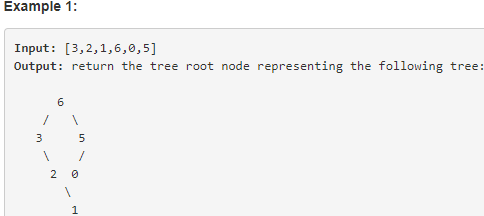
\includegraphics[width=0.6\textwidth]{example654.png}
\caption{Q654 Given Example}
\end{figure} \\
For us this did not make it any clearer as to which way we should structure the subtrees. We were able to understand that the biggest number of each subarray should be the next number and work down in a descending order from the root. We were unable to understand why the 2 was to the right of 3, and yet 0 was to the left of 5. This confusion did cause us to take longer to solve this question than anticipated.

\section{Conclusion}
\bibliography{mybib}
\bibliographystyle{ieeetr}

\end{document}